\subsection{What is metamaterial}

\begin{frame}{What is metamaterial?}
    \begin{columns}
        \column{0.5\textwidth}
        Metamaterials:
        \begin{itemize}
            \item Properties depend on structure.
            \item Usually based on periodic structure.
        \end{itemize}
        \vspace{1mm}
        Unusual properties and applications:
        \begin{itemize}
            \item Negative permittivity and permeability.
            \item Perfect absorber.
            \item Perfect lens.
            \item Bending waves.
            \item ...
        \end{itemize}
        \column{0.5\textwidth}
        \begin{figure}
            \centering
            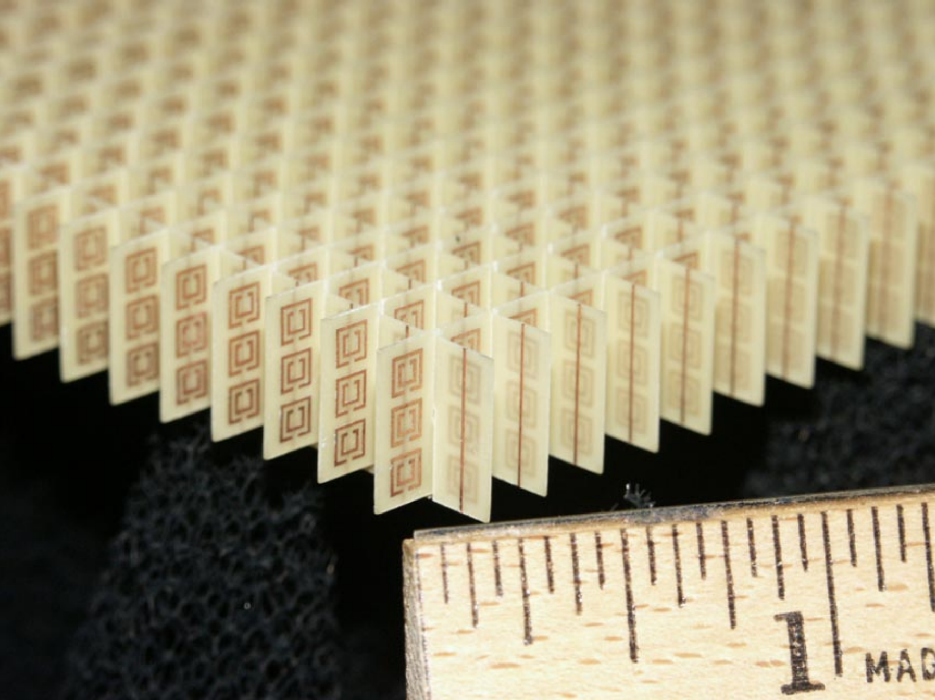
\includegraphics[width=\textwidth]{Figures/Meta_DN.pdf}
            \caption{Periodic structure. \cite{10.1063/1.1850590}}
            \label{fig:Periodic_structure}
        \end{figure}
    \end{columns}
\end{frame}